\section{Principal Component Analysis \hpoints{25}}

In this exercise, you will use a part of the MNIST digit dataset, which consists of examples of handwritten digits. Training data is provided in \(\mathtt{MNIST\_train.mat}\) and test data in \(\mathtt{MNIST\_test.mat}\). Each example is a $28 \times 28$ grayscale image, which leads to $784$ pixels to use as features. Each of the labels is shifted by $1$, i.e. the label for the digit '$0$' is $1$ and so on.

You will use PCA to reduce the training data (the pixel data of the training set) from 784 dimensions to 100 dimensions. To 
answer the questions you need to write code in MATLAB to process
the dataset. You {\bf are} allowed to use built-in MATLAB functions for PCA, K-means, fitgmdist, etc. for this problem.

\begin{enumerate}

\item \points{5} Using the top 2 PCA dimensions, display all the test
  digits ``0'' and ``1'', using circles and crosses respectively.
  An example of a plot of ``3'' vs ``4'' is shown in Figure. 1 below. All correct axes, title, and legend must be included.
  Note that the sign of loadings are abitrary (i.e. [-1,1] is the same as [1,-1]).

  \begin{figure}[h!]
    \centering
    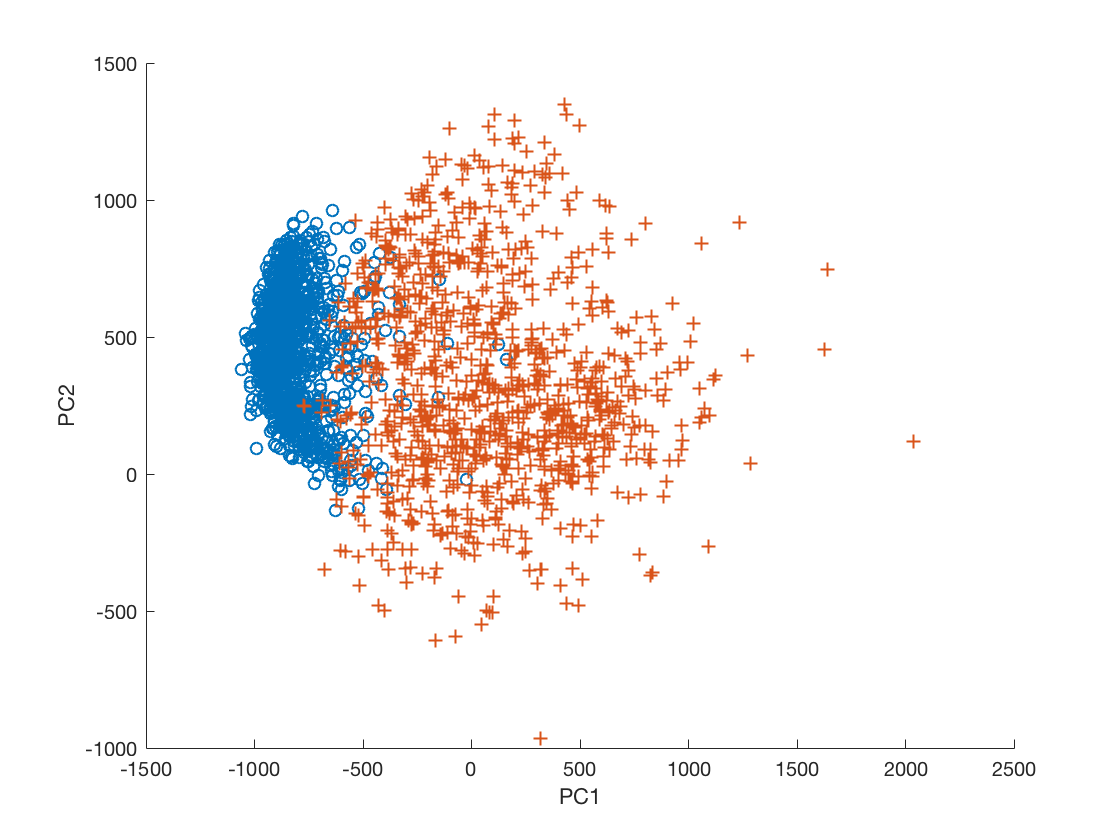
\includegraphics[width=0.65\textwidth]{images/pca_2_vs_3}
    \caption{Plot of '2'-'3' digits from top 2 PCA
        dimensions}\label{fig:pca_2_vs_3}
  \end{figure}
  

\item \points{5} Plot the average (in sample) reconstruction error  $||X - \hat{X}||_F^2$
of the digits as a function of the number of principle components that are included.  How many
principal components are required to get 85\% reconstruction accuracy? (i.e., to explain 85\% of the 
variance: $||\hat{X}-\bar{X}||_F^2/ ||X - \bar{X}||_F^2 = 0.85$ where $\bar{X}$ is a matrix, every row of which is the
average $x$ -- the average image)  
Reminder: make sure you understand the MATLAB function you used, especially whether the function standardize the dataset before running PCA 
and please state it clearly in your solution.


\item \points{10} Cluster the data into 10 clusters using k-means and assign a digit to each cluster.
Report the accuracy on the test set using 100, 150 and 200 top dimensions.
Also state that whether the method you use standardizes the dataset. 

\textbf{Notes:}
  \begin{itemize} 
  \item Please use the following class assignment rule: count the class labels in each cluster, and choose the most popular class (mode) as the label for that cluster.
  \item You can use MATLAB's builtin \(\mathtt{pca}\) and \(\mathtt{kmeans}\) functions. Please read the documentation and understand how to use them.
  \item Both the PCA and the k-means should be trained only on the training set.
  \end{itemize}

\item \points{2} What is the major drawback with the above method, and please name one way to improve it?


\item \points{3} Rerun the above algorithm with 25 clusters using 100, 150, and 200 top dimensions and report the accuracy on the test set. Again, state whether your method standardizes the dataset.

  
\end{enumerate}
